\documentclass[a4paper, 12pt]{article}
\usepackage[utf8]{inputenc}
\usepackage[T1]{fontenc}
\usepackage[top=2.5cm, bottom=2.5cm, left=3cm, right=2.5cm]{geometry}
\usepackage{graphicx}
\usepackage{nopageno}
\usepackage{setspace}
\usepackage{amsmath}
\usepackage{titlesec}
\usepackage{array}
\usepackage{booktabs}
\usepackage{multirow}
\usepackage{float}
\usepackage{url}
\IfFileExists{newtxtext.sty}{%
    \usepackage{newtxtext,newtxmath}%
}{%
    \usepackage{mathptmx}%
}
\usepackage{multicol}
\usepackage[labelsep=period,skip=4pt]{caption}
\usepackage{indentfirst}
\usepackage{enumitem}
\usepackage{longtable}
\usepackage{tabularx}
\usepackage{siunitx}
\usepackage{pgfplots}
\usepackage{tikz}
\usepackage{xcolor}
\usepackage{listings}
\usepackage{hyperref}

\pgfplotsset{compat=1.16}
\usetikzlibrary{arrows.meta,positioning,calc}
\sisetup{
    output-decimal-marker={,},
    group-separator={.},
    group-digits=integer,
    range-phrase={--},
    range-units=single,
    detect-all,
    per-mode=symbol
}
\hypersetup{
    colorlinks=true,
    linkcolor=black,
    citecolor=black,
    urlcolor=black,
    hypertexnames=false,
    pdftitle={Laporan Audit Instrumentasi Group I - FIT310},
    pdfauthor={Group I}
}

% 1. Paragraph & spacing setting (Template O2)
\linespread{1.25}
\setlength{\parindent}{0.8cm}
\setstretch{1.25}
\setlength{\columnsep}{10pt}
\setlength{\parskip}{0pt}

\setlength{\textfloatsep}{6pt}
\setlength{\intextsep}{6pt}
\setlength{\floatsep}{6pt}

\titlespacing*{\section}{0pt}{8pt}{4pt}
\titlespacing*{\subsection}{0pt}{0.4em}{0.2em}
\titlespacing*{\subsubsection}{0pt}{0.3em}{0.15em}

\setlist[enumerate]{
    itemsep=2pt,
    parsep=0pt,
    topsep=0pt,
    partopsep=0pt
}
\setlist[itemize]{
    itemsep=2pt,
    parsep=0pt,
    topsep=0pt,
    partopsep=0pt
}

% 2. Figure and Table Setting
\renewcommand{\figurename}{Gambar}
\renewcommand{\tablename}{Tabel}

% 3. Pengaturan Section (Polosan, tanpa huruf/nomor) - Template O2
\renewcommand{\thesection}{}
\titleformat{\section}
{\normalfont\bfseries}{}{0pt}{}

% 4. Pengaturan Subsection (Format: a. Judul) - Template O2
\renewcommand{\thesubsection}{\alph{subsection}.}
\titleformat{\subsection}
{\normalfont\bfseries}{\thesubsection}{0.5em}{}

\renewcommand{\thesubsubsection}{}
\titleformat{\subsubsection}
{\normalfont\bfseries}{}{0pt}{}

% 5. Listing kode untuk Lampiran
\lstset{
    basicstyle=\ttfamily\footnotesize,
    breaklines=true,
    frame=single,
    columns=fullflexible,
    keepspaces=true,
    showstringspaces=false,
    xleftmargin=0.2cm
}

% 6. Makro metrologi
\newcommand{\uc}{u_{c}}
\newcommand{\uA}{u_{A}}
\newcommand{\uB}{u_{B}}
\newcommand{\dd}{\mathrm{d}}

% 7. Pustaka / Bibliografi (Template O2)
\usepackage{csquotes}
\IfFileExists{biblatex.sty}{%
    \usepackage[style=apa,sortcites=true,sorting=nyt,backend=biber]{biblatex}
    \DeclareLanguageMapping{american}{american-apa}
    \addbibresource{Pustaka.bib}
    \setlength{\bibitemsep}{0.0\baselineskip}
}{%
    \usepackage[numbers,sort&compress]{natbib}
    \bibliographystyle{apalike}
    \renewcommand{\bibsection}{}
    \setlength{\bibsep}{2pt}
    \newcommand{\printbibliography}[1][]{\footnotesize\bibliography{Pustaka}}
    \providecommand{\parencite}{\citep}
}

\hypersetup{
    pdftitle={Laporan Kalibrasi Instrumentasi dan Evaluasi Metrologis - Universitas Airlangga},
    pdfauthor={Group I - Departemen Fisika UNAIR}
}

\begin{document}
    \begin{titlepage}
    \begin{center}
        % Judul
        \textbf{LAPORAN KALIBRASI INSTRUMENTASI DAN EVALUASI METROLOGIS}\\[0.0\baselineskip]
        \textbf{PROYEK ELABORATIF PENGUKURAN FISIKA BERBASIS KASUS}\\[0.0\baselineskip]
        \textbf{``KETEPATAN DAN KETIDAKPASTIAN DALAM PRAKTIKUM NYATA''}\\[0.0\baselineskip]
        \textbf{EKSPERIMEN P1 (DENSITY) DAN M3 (ENERGY)}\\[0.5\baselineskip]

        % Ruler
        \hrule height 2pt
        \vspace{0.5\baselineskip}

        % Mata Kuliah, Tanggal, dan Kelompok
        {\footnotesize
        \begin{tabular*}{\textwidth}{@{\extracolsep{\fill}} l c r @{}}
            Mata Kuliah: Sensor dan Pengukuran (FIT310) & Tanggal: 17 November 2026 & Kelompok: Group I
        \end{tabular*}
        }
        \vspace{2\baselineskip}

        \begin{figure}[H]
            \centering
            
\includegraphics[width=6cm, height=6cm]{Images/logo-unair.png}
        \end{figure}
        \vspace{1\baselineskip}

        \begin{table}[H]
            \centering
            \renewcommand{\arraystretch}{1.05}{
                \begin{tabular}{lc}
                    \multicolumn{2}{c}{\textbf{Disusun Oleh (Group I)}} \\
                    Muhammad Abiyu Khansa & (182241036) \\
                    Farras Atha Pandita & (182241040) \\
                    Hendra Maulana & (182241043)
                \end{tabular}}
        \end{table}

        \textbf{Dosen Pembina :} \\
        \centering
        Winarno, S.Si., M.T. (Pertemuan 1--7) \\
        Yhosep Gita Yhun Yhuwana, S.Si., M.T. (Pertemuan 8--14)

        \vfill
        \begin{center}
            \textbf{PROGRAM STUDI FISIKA \\
                    DEPARTEMEN FISIKA \\
                    FAKULTAS SAINS DAN TEKNOLOGI \\
                    UNIVERSITAS AIRLANGGA \\
                    2026}
        \end{center}
    \end{center}
\end{titlepage}

    \begin{center}
    \underline{\textbf{KALIBRASI INSTRUMENTASI DAN EVALUASI METROLOGIS:}} \\
    \underline{\textbf{KETEPATAN DAN KETIDAKPASTIAN PADA EKSPERIMEN}} \\
    \underline{\textbf{P1 (\textit{DENSITY}) DAN M3 (\textit{ENERGY})}}
\end{center}

\begin{center}
    Muhammad Abiyu Khansa (182241036), Farras Atha Pandita (182241040), Hendra Maulana (182241043)
\end{center}

\hrule height 2pt

\begin{center}
    \textbf{Program Studi Fisika, Departemen Fisika, Fakultas Sains dan Teknologi, Universitas Airlangga, Surabaya}
\end{center}

\vspace{10pt}
\renewcommand{\abstractname}{\normalsize{ABSTRAK}}
\begin{abstract}
\noindent
Laporan ini memuat hasil kalibrasi instrumentasi dan evaluasi metrologis pada dua eksperimen fisika, yaitu P1 (massa jenis silinder kuningan) dan M3 (konservasi energi mekanik pada rel udara). Sesuai ketentuan kelompok beranggotakan tiga orang, setiap besaran diukur sebanyak $n=8$ kali. Penapisan pencilan dengan kriteria $3\sigma$ tidak membuang satu pun data. Ketidakpastian dievaluasi menurut ISO-GUM (Tipe A dan Tipe B, $\uc$, dan $U$ pada $k=2$). Hasil P1 adalah $\rho=(8{,}493\pm0{,}035)\ \si{g/cm^3}$ dengan kontribusi ketidakpastian terbesar berasal dari diameter ($85\%$). Kalibrasi neraca digital terhadap $8$ titik massa standar menghasilkan $y=0{,}999975\,x+0{,}0421$ dengan $R^2\approx 1$, tetapi plot residual menunjukkan pola lengkung sistematis (simpangan maksimum $0{,}032\ \si{g}$) sehingga $R^2$ saja tidak cukup sebagai bukti linearitas. Pada M3 diperoleh $\Delta E=E_1-E_2=(-2{,}79\pm0{,}61)\times10^{-3}\ \si{J}$; tanda negatif berarti energi akhir lebih besar daripada energi awal, yang secara fisis tidak mungkin pada sistem disipatif. Hasil ini ditafsirkan sebagai indikasi galat sistematis (terutama \textit{response time delay} sensor gerbang cahaya) dan bukan sebagai pelanggaran hukum kekekalan energi.
\end{abstract}

\vspace{5pt}
\noindent\textbf{Kata kunci:} kalibrasi instrumentasi, ISO-GUM, ketidakpastian bentangan, regresi OLS, analisis residual, massa jenis, kekekalan energi, rel udara.


%======== Bagian Inti ===========
\newpage
\begin{multicols}{2}
    \raggedcolumns
    \section{PENDAHULUAN}
        \subsection{Latar Belakang}
        Laboratorium Fisika Dasar menerima satu \textit{batch} instrumen dan sensor baru, antara lain neraca digital, jangka sorong, rel udara dengan sensor gerak (gerbang cahaya), osiloskop, dan termometer digital. Ketika \textit{batch} ini digunakan pada eksperimen yang identik oleh beberapa kelompok praktikan, muncul penyimpangan data yang berbeda-beda antar-instrumen. Penyimpangan tersebut dapat berasal dari histeresis dan gesekan mekanis, gangguan lingkungan (\textit{modifying inputs}), \textit{noise} sinyal, efek pembebanan sistem (\textit{loading effect}), atau galat paralaks dan resolusi digital \parencite{Bentley2005}.

        Dalam kondisi tersebut kelompok ditunjuk sebagai Tim Evaluasi dan Kalibrasi Instrumentasi. Tugasnya adalah menentukan apakah penyimpangan berasal dari cacat internal instrumen, kesalahan kalibrasi, \textit{loading effect}, gangguan lingkungan, atau ketidakpastian acak \parencite{WinarnoYhuwana}. Group I mendapat pasangan eksperimen \textbf{P1 (\textit{Density})} dan \textbf{M3 (\textit{Energy})} dengan fokus pada data statis dan dinamis serta respon sensor gerak. Karena kelompok beranggotakan tiga orang, jumlah pengulangan dikurangi $25\%$ menjadi $n=8$ per besaran, tanpa mengurangi kedalaman analisis.

        \subsection{Rumusan Masalah}
        Rumusan masalah evaluasi ini adalah sebagai berikut:
        \begin{enumerate}
            \item Bagaimana karakteristik statis dan dinamis instrumen yang digunakan pada eksperimen P1 dan M3?
            \item Bagaimana hasil kalibrasi neraca digital terhadap massa standar dan apakah sebaran residualnya menunjukkan linearitas yang sebenarnya?
            \item Berapa ketidakpastian gabungan ($\uc$) dan ketidakpastian bentangan ($U$, $k=2$) untuk massa jenis $\rho$ dan penyusutan energi mekanik $\Delta E$?
            \item Bagaimana dampak keterbatasan instrumen terhadap kesimpulan ilmiah mengenai massa jenis dan hukum kekekalan energi mekanik?
        \end{enumerate}

        \subsection{Tujuan Evaluasi}
        \begin{enumerate}
            \item Memetakan parameter kinerja instrumen: \textit{measurand}, \textit{range}, resolusi, sensitivitas, akurasi, presisi, \textit{repeatability}, linearitas, \textit{response time}, stabilitas, dan \textit{noise} \parencite{JCGM2012VIM}.
            \item Menjalankan kalibrasi terstruktur terhadap standar acuan, memodelkan regresi $y=ax+b$, dan mengevaluasi grafik residual.
            \item Menghitung $\uA$, $\uB$, $\uc$, dan $U$ ($k=2$, tingkat kepercayaan sekitar $95\%$) serta menerapkan aturan angka penting sesuai ISO-GUM \parencite{JCGM2008GUM}.
            \item Menyusun analisis reflektif \textit{``so what?''} dan rekomendasi kalibrasi teknis.
        \end{enumerate}

        \subsection{Profil Instrumen}
        Instrumen yang dievaluasi beserta spesifikasi yang dipakai pada perhitungan dirangkum pada Tabel~\ref{tab:profil}.
\end{multicols}

%=== Tabel Profil Instrumen (Full Width) ===
\begin{table}[H]
\centering
\singlespacing
\caption{Profil instrumen yang dievaluasi (Group I).}
\label{tab:profil}
\small
\begin{tabularx}{\textwidth}{@{}l l X l@{}}
\toprule
\textbf{Eksperimen} & \textbf{Instrumen} & \textbf{\textit{Measurand}} & \textbf{Resolusi}\\
\midrule
P1 & Neraca digital (0--500 g) & Massa silinder kuningan $m$ & \SI{0,01}{g}\\
P1 & Jangka sorong & Diameter $d$ dan tinggi $h$ silinder & \SI{0,05}{mm}\\
M3 & Neraca digital & Massa \textit{glider} $M$ & \SI{0,01}{g}\\
M3 & Jangka sorong & Lebar \textit{flag} $w$ & \SI{0,05}{mm}\\
M3 & Penggaris/pengukur tinggi & Beda ketinggian $\Delta h$ & \SI{0,1}{mm}\\
M3 & Gerbang cahaya + \textit{timer} digital & Waktu interupsi $\Delta t_1$, $\Delta t_2$ & \SI{0,1}{ms}\\
Kalibrasi & Anak timbangan standar kelas F2 & Massa acuan $x$ (10--300 g) & $u_{\mathrm{std}}\le\SI{0,002}{g}$\\
\bottomrule
\end{tabularx}
\end{table}

\begin{multicols}{2}
    \raggedcolumns
    \section{METODE DAN DATA EKSPERIMEN}
        \subsection{Skema dan Prosedur Eksperimen P1 (Massa Jenis)}
        Massa jenis silinder kuningan ditentukan secara tidak langsung dari tiga besaran terukur \parencite{HallidayResnickWalker}:
        \begin{equation}
            \rho=\frac{m}{V}=\frac{4m}{\pi d^{2}h}.
            \label{eq:rho}
        \end{equation}
        Prosedur pelaksanaannya meliputi: (1) neraca digital di-nol-kan pada permukaan rata dan tidak bergetar; (2) massa silinder diukur $n=8$ kali; (3) diameter dan tinggi silinder diukur $n=8$ kali dengan jangka sorong pada posisi yang divariasikan; (4) data ditapis dengan kriteria $3\sigma$; serta (5) nilai rata-rata dan ketidakpastian dihitung, lalu dirambatkan ke $\rho$.

        \subsection{Skema dan Prosedur Eksperimen M3 (Energi pada Rel Udara)}
        Sebuah \textit{glider} bermassa $M$ dengan \textit{flag} selebar $w$ meluncur di atas rel udara miring melewati dua gerbang cahaya (Gambar~\ref{fig:skema}). Posisi gerbang~1 berada pada $x_1=\SI{30}{cm}$ dengan ketinggian acuan $\Delta h=\SI{28}{mm}$ di atas gerbang~2, dan gerbang~2 berada pada $x_2=\SI{110}{cm}$ (jarak $\Delta s=\SI{0,80}{m}$). Kecepatan pada tiap gerbang dihitung dari:
        \begin{equation}
            v_i=\frac{w}{\Delta t_i},\qquad i=1,2,
            \label{eq:v}
        \end{equation}
        dan energi mekanik total pada tiap posisi (gravitasi lokal $g=\SI{9,806}{m/s^2}$) adalah \parencite{HallidayResnickWalker}:
        \begin{equation}
            \begin{aligned}
                E_1 &= \tfrac{1}{2}Mv_1^{2}+Mg\,\Delta h, \\
                E_2 &= \tfrac{1}{2}Mv_2^{2},\qquad \Delta E=E_1-E_2.
            \end{aligned}
            \label{eq:E}
        \end{equation}
        Jika energi mekanik kekal dan tidak ada disipasi maka $\Delta E=0$. Jika ada gesekan dan hambatan udara maka diharapkan $\Delta E>0$.
\end{multicols}

%=== Gambar Skema Eksperimen M3 (Full Width) ===
\begin{figure}[H]
\centering
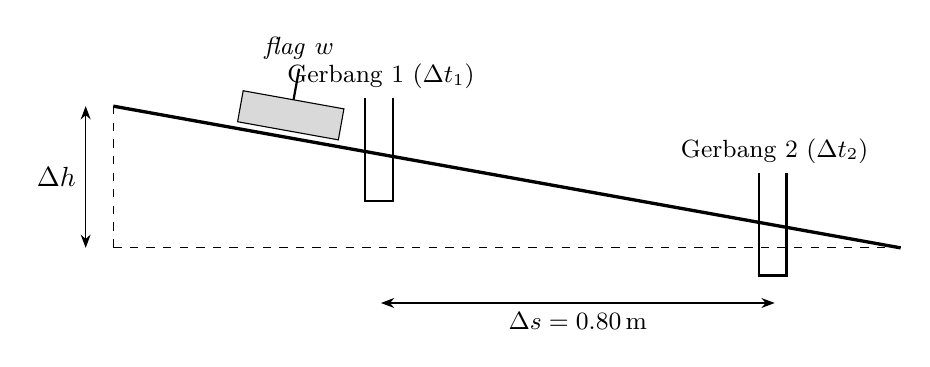
\begin{tikzpicture}[>=Stealth,scale=1.0]
  % rel miring
  \draw[very thick] (0,2.2) -- (10,0.4);
  \draw[dashed] (0,0.4) -- (10,0.4);
  \draw[dashed] (0,2.2) -- (0,0.4);
  \draw[<->] (-0.35,0.4) -- (-0.35,2.2) node[midway,left]{$\Delta h$};
  % glider
  \begin{scope}[rotate=-10.2,shift={(1.2,2.2)}]
    \fill[gray!30,draw=black] (0,0.05) rectangle (1.3,0.45);
    \draw[thick] (0.65,0.45) -- (0.65,0.85);
    \node[above] at (0.65,0.85) {\small \textit{flag} $w$};
  \end{scope}
  % gerbang 1
  \draw[thick] (3.2,2.3) -- (3.2,1.0) -- (3.55,1.0) -- (3.55,2.3);
  \node[above] at (3.4,2.3) {\small Gerbang 1 ($\Delta t_1$)};
  % gerbang 2
  \draw[thick] (8.2,1.35) -- (8.2,0.05) -- (8.55,0.05) -- (8.55,1.35);
  \node[above] at (8.4,1.35) {\small Gerbang 2 ($\Delta t_2$)};
  \draw[<->] (3.4,-0.3) -- (8.4,-0.3) node[midway,below]{\small $\Delta s=\SI{0,80}{m}$};
\end{tikzpicture}
\caption{Skema eksperimen M3: \textit{glider} pada rel udara miring dengan dua gerbang cahaya.}
\label{fig:skema}
\end{figure}

\begin{multicols}{2}
    \raggedcolumns
        \subsection{Data Mentah P1 dan M3 (\texorpdfstring{$n=8$}{n=8})}
        Seluruh data mentah eksperimen P1 (silinder kuningan) dan M3 (rel udara) dicatat tanpa pembulatan awal sebagaimana disajikan pada Tabel~\ref{tab:p1} dan Tabel~\ref{tab:m3}.

        \subsection{Penapisan Pencilan Kriteria \texorpdfstring{$3\sigma$}{3 sigma}}
        Suatu data dinyatakan pencilan bila $|x_i-\bar{x}|>3\sigma$ \parencite{Taylor1997}. Hasil penapisan pada semua besaran ditunjukkan pada Tabel~\ref{tab:z}. Seluruh data lolos, sehingga tidak ada data yang dibuang dan $n=8$ dipakai penuh.

        Perlu dicatat bahwa untuk sampel kecil, kriteria ini secara matematis tidak dapat menandai pencilan bila $\sigma$ diambil dari sampel itu sendiri. Simpangan standar-terbesar yang mungkin dicapai satu data adalah $(n-1)/\sqrt{n}=7/\sqrt{8}\approx 2{,}47$ simpangan baku sampel, yang selalu lebih kecil dari $3$. Dengan demikian lolosnya semua data bukan bukti kuat bahwa data bebas pencilan. Kebersihan data didukung oleh nilai simpangan baku yang kecil dan tidak adanya nilai yang menyimpang jauh secara visual.
\end{multicols}

%=== Tabel Data Mentah P1 & M3 (Full Width) ===
\begin{table}[H]
\centering
\singlespacing
\caption{Data mentah P1 (silinder kuningan, $n=8$) beserta status penapisan $3\sigma$.}
\label{tab:p1}
\small
\begin{tabular}{c S[table-format=2.2] c S[table-format=2.2] c S[table-format=2.2] c}
\toprule
\textbf{Trial} & {\textbf{Massa (g)}} & \textbf{Status} & {\textbf{Diameter (mm)}} & \textbf{Status} & {\textbf{Tinggi (mm)}} & \textbf{Status} \\
\midrule
1 & 67.22 & Lolos & 20.05 & Lolos & 25.10 & Lolos \\
2 & 67.21 & Lolos & 20.00 & Lolos & 25.15 & Lolos \\
3 & 67.23 & Lolos & 20.05 & Lolos & 25.10 & Lolos \\
4 & 67.20 & Lolos & 20.10 & Lolos & 25.05 & Lolos \\
5 & 67.24 & Lolos & 20.00 & Lolos & 25.10 & Lolos \\
6 & 67.22 & Lolos & 20.05 & Lolos & 25.15 & Lolos \\
7 & 67.21 & Lolos & 20.00 & Lolos & 25.10 & Lolos \\
8 & 67.23 & Lolos & 20.05 & Lolos & 25.05 & Lolos \\
\bottomrule
\end{tabular}
\end{table}

\begin{table}[H]
\centering
\singlespacing
\caption{Data mentah M3 (rel udara, $n=8$) beserta status penapisan $3\sigma$.}
\label{tab:m3}
\small
\begin{tabular}{c S[table-format=1.4] c S[table-format=1.4] c S[table-format=3.2] S[table-format=2.2] S[table-format=2.1]}
\toprule
\textbf{Trial} & {$\Delta t_1$ (s)} & \textbf{Status} & {$\Delta t_2$ (s)} & \textbf{Status} & {$M$ (g)} & {$w$ (mm)} & {$\Delta h$ (mm)} \\
\midrule
1 & 0.0521 & Lolos & 0.0278 & Lolos & 200.10 & 25.00 & 28.0 \\
2 & 0.0519 & Lolos & 0.0279 & Lolos & 200.12 & 25.05 & 28.1 \\
3 & 0.0523 & Lolos & 0.0277 & Lolos & 200.08 & 25.00 & 28.0 \\
4 & 0.0520 & Lolos & 0.0280 & Lolos & 200.11 & 24.95 & 27.9 \\
5 & 0.0522 & Lolos & 0.0278 & Lolos & 200.09 & 25.00 & 28.0 \\
6 & 0.0518 & Lolos & 0.0279 & Lolos & 200.10 & 25.05 & 28.1 \\
7 & 0.0524 & Lolos & 0.0277 & Lolos & 200.13 & 25.00 & 28.0 \\
8 & 0.0521 & Lolos & 0.0278 & Lolos & 200.07 & 24.95 & 27.9 \\
\bottomrule
\end{tabular}
\end{table}


%=== Tabel Simpangan Z-max (Full Width) ===
\begin{table}[H]
\centering
\singlespacing
\caption{Simpangan terbesar terhadap rata-rata dalam satuan $s$ ($z_{\max}=\max|x_i-\bar{x}|/s$).}
\label{tab:z}
\small
\begin{tabular}{l c c}
\toprule
\textbf{Besaran} & $z_{\max}$ & \textbf{Hasil ($z_{\max}<3$)}\\
\midrule
Massa $m$ (P1) & 1,53 & Semua lolos\\
Diameter $d$ & 1,77 & Semua lolos\\
Tinggi $h$ & 1,32 & Semua lolos\\
Waktu $\Delta t_1$ & 1,50 & Semua lolos\\
Waktu $\Delta t_2$ & 1,69 & Semua lolos\\
Massa \textit{glider} $M$ & 1,50 & Semua lolos\\
Lebar \textit{flag} $w$ & 1,32 & Semua lolos\\
Beda tinggi $\Delta h$ & 1,32 & Semua lolos\\
\bottomrule
\end{tabular}
\end{table}

\begin{multicols}{2}
    \raggedcolumns
    \section{ANALISIS KARAKTERISTIK ALAT UKUR}
        \subsection{Rangkuman Parameter Statis dan Dinamis}
        Tabel~\ref{tab:param} merangkum parameter kinerja metrologis yang dapat ditetapkan dari data evaluasi \parencite{JCGM2012VIM,MorrisLangari}. Nilai yang belum diukur langsung diberi keterangan.
\end{multicols}

%=== Tabel Parameter Performa (Full Width) ===
\begin{table}[H]
\centering
\singlespacing
\caption{Parameter performa metrologi neraca digital dan sensor gerak.}
\label{tab:param}
\small
\begin{tabularx}{\textwidth}{@{}l l X@{}}
\toprule
\textbf{Parameter} & \textbf{Kategori} & \textbf{Hasil evaluasi}\\
\midrule
\textit{Measurand} & Statis/Dinamis & Massa (g), panjang (mm), waktu interupsi (s)\\
\textit{Range} & Statis & Neraca \SIrange{0}{500}{g}; jangka sorong \SIrange{0}{150}{mm}\\
Resolusi & Statis & Neraca \SI{0,01}{g}; jangka sorong \SI{0,05}{mm}; \textit{timer} \SI{0,1}{ms}\\
Sensitivitas & Statis & $S=a=0{,}999975\ \si{g/g}$ (ideal $1{,}000000$)\\
Akurasi & Statis & Bias rata-rata $\bar{m}-m_{\mathrm{ref}}=\SI{0,020}{g}$ ($0{,}030\%$) terhadap acuan \SI{67,20}{g}\\
Presisi & Statis & $s_m=\SI{0,0131}{g}$ ($n=8$)\\
\textit{Repeatability} & Statis & $r=2{,}8\,s_r=\SI{0,037}{g}$\\
Linearitas & Statis & Simpangan maks. dari garis OLS $\SI{0,032}{g}$ ($0{,}011\%$ \textit{full scale} \SI{300}{g}); residual berpola lengkung\\
\textit{Response time} & Dinamis & Tunda optoelektronik gerbang cahaya $\tau\approx\SI{0,8}{ms}$ (\textit{rise} $\approx\SI{20}{\micro s}$, \textit{fall} $\approx\SI{35}{\micro s}$); nilai ini adalah asumsi dari spesifikasi sensor yang dipakai pada perhitungan dan belum diverifikasi dengan osiloskop\\
Stabilitas & Statis/Dinamis & \textit{Zero drift} neraca $+\SI{0,03}{g}$ dalam $30$ menit (Tabel~\ref{tab:drift})\\
\textit{Noise} & Statis/Dinamis & Fluktuasi acak neraca setara $s_m=\SI{0,013}{g}$, atau sekitar $1$ digit resolusi\\
\bottomrule
\end{tabularx}
\end{table}

\begin{multicols}{2}
    \raggedcolumns
        \subsection{Karakteristik Statis (Eksperimen P1)}
            \subsubsection{Akurasi dan Galat}
            Dengan $E_m=\bar{m}=\SI{67,22}{g}$ dan $E_o=\SI{67,20}{g}$:
            \begin{align}
                E_{\mathrm{abs}} &= |E_m-E_o|=\SI{0,020}{g},\\
                E_{\mathrm{rel}} &= \frac{|E_m-E_o|}{E_o}=2{,}98\times10^{-4},\\
                \%E &= 0{,}030\%.
            \end{align}
            Bias ini sama dengan dua kali resolusi neraca. Karena $E_{\mathrm{abs}}=\SI{0,020}{g}$ lebih besar daripada ketidakpastian bentangan massa $U_m=\SI{0,011}{g}$, bias ini signifikan secara metrologis dan sejalan dengan galat penguatan (\textit{gain}) yang terlihat pada analisis kalibrasi.

            \subsubsection{Repeatability dan Zero Drift}
            Simpangan baku sampel massa $s_r=\SI{0,0131}{g}$ memberikan batas \textit{repeatability} $r=2{,}8\,s_r=\SI{0,037}{g}$. Uji \textit{zero drift} neraca tanpa beban setelah pembebanan siklik tercatat pada Tabel~\ref{tab:drift}.

            Pergeseran nol sebesar $\SI{0,03}{g}$ dalam $30$ menit (laju sekitar $\SI{1e-3}{g/menit}$) setara tiga langkah resolusi. Penyebabnya diduga \textit{creep} mekanik sel beban (\textit{strain gauge}) dan \textit{drift} termal pada penguat/ADC. Praktiknya, neraca perlu di-nol-kan ulang (tombol \textit{tare}) sebelum tiap rangkaian pengukuran \parencite{MorrisLangari}.

        \subsection{Karakteristik Dinamis dan Efek Pembebanan (Eksperimen M3)}
            \subsubsection{Response Time Delay Gerbang Cahaya}
            Komparator pada gerbang cahaya memiliki histeresis yang menimbulkan waktu tunda $\tau$. Pemodelan yang dipakai adalah $\Delta t_{\mathrm{ukur}}=\Delta t_{\mathrm{sejati}}-\tau$, sehingga kecepatan terukur sedikit terlalu besar. Dengan $\tau=\SI{0,8}{ms}$ dan waktu rata-rata $\overline{\Delta t_1}=\SI{52,10}{ms}$ serta $\overline{\Delta t_2}=\SI{27,825}{ms}$ diperoleh hasil pada Tabel~\ref{tab:delay}.

            Bias relatif pada gerbang~2 hampir dua kali lipat karena waktu interupsinya lebih pendek, sehingga $\tau$ yang tetap menjadi bagian relatif yang lebih besar ($\tau/\Delta t$). Ini ciri khas galat sistematis, yaitu tidak berkurang dengan memperbanyak pengulangan \parencite{Taylor1997}.

            \subsubsection{Loading Effect dan Model Th\'evenin}
            Efek pembebanan sistem dimodelkan dengan rangkaian ekuivalen Th\'evenin \parencite{Bentley2005}:
            \begin{equation}
                \frac{E_m}{E_o}=\frac{R_m}{R_{AB}+R_m}.
                \label{eq:thevenin}
            \end{equation}
            Agar $E_m/E_o\approx1$ diperlukan $R_m\gg R_{AB}$. Misalnya, untuk galat pembebanan di bawah $1\%$ diperlukan $R_m\ge 99\,R_{AB}$. Pada rel udara, \textit{loading effect} bersifat analogi mekanis: gesekan lapisan batas udara dan pengereman arus pusar pasif (\textit{eddy current}) berperan sebagai ``hambatan dalam'' $R_{AB}$ yang menyerap sebagian energi sehingga besaran yang terukur menyimpang dari nilai sejati. Persamaan~\eqref{eq:thevenin} dipakai di sini sebagai kerangka konseptual dan bukan sebagai model kuantitatif karena nilai $R_{AB}$ mekanis tidak diukur dalam eksperimen ini.

            \subsubsection{Modifying Inputs}
            Embusan udara dari ventilasi/AC laboratorium memodifikasi gaya hambat aerodinamis pada \textit{glider}, dan kemiringan rel yang tidak persis terkalibrasi mengubah $\Delta h$ efektif. Kedua hal ini bukan galat alat melainkan gangguan lingkungan yang masuk ke \textit{measurand} \parencite{Bentley2005}.
\end{multicols}

%=== Tabel Zero Drift & Response Delay (Full Width) ===
\begin{table}[H]
\centering
\singlespacing
\caption{Uji \textit{zero drift} neraca digital tanpa beban.}
\label{tab:drift}
\small
\begin{tabular}{l *{7}{S[table-format=1.2]}}
\toprule
Waktu (menit) & {0} & {5} & {10} & {15} & {20} & {25} & {30}\\
Pembacaan nol (g) & 0.00 & 0.00 & 0.01 & 0.01 & 0.02 & 0.02 & 0.03\\
\bottomrule
\end{tabular}
\end{table}

\begin{table}[H]
\centering
\singlespacing
\caption{Efek \textit{response time delay} $\tau=\SI{0,8}{ms}$ pada kecepatan.}
\label{tab:delay}
\small
\begin{tabular}{l S[table-format=1.4] S[table-format=1.4] S[table-format=1.2]}
\toprule
\textbf{Gerbang} & {$v_{\mathrm{ukur}}$ (m/s)} & {$v_{\mathrm{terkoreksi}}$ (m/s)} & {Bias (\%)}\\
\midrule
1 & 0.4798 & 0.4726 & 1.54\\
2 & 0.8985 & 0.8734 & 2.88\\
\bottomrule
\end{tabular}
\end{table}

\begin{multicols}{2}
    \raggedcolumns
    \section{PERHITUNGAN KETIDAKPASTIAN DAN GALAT}
        \subsection{Formulasi ISO-GUM}
        Evaluasi ketidakpastian standar Tipe A ($\uA$), Tipe B ($\uB$), gabungan ($\uc$), dan bentangan ($U$) mengikuti pedoman ISO-GUM \parencite{JCGM2008GUM}:
        \begin{align}
            \uA &= \frac{s}{\sqrt{n}},\quad s=\sqrt{\frac{\sum_{i=1}^{n}(x_i-\bar{x})^2}{n-1}},\label{eq:uA}\\
            \uB &= \frac{\text{Resolusi}}{2\sqrt{3}},\label{eq:uB}\\
            \uc &= \sqrt{\uA^{2}+\uB^{2}},\quad U=k\,\uc=2\,\uc.\label{eq:U}
        \end{align}
        Untuk besaran turunan $f(x_1,\dots,x_N)$ dipakai hukum perambatan ketidakpastian:
        \begin{equation}
            \uc(f)=\sqrt{\sum_{i=1}^{N}\left(\frac{\partial f}{\partial x_i}\right)^{2}\uc^{2}(x_i)}.
            \label{eq:prop}
        \end{equation}
        Nilai akhir dilaporkan dengan $U$ dibulatkan ke dua angka penting dan nilai rata-rata dibulatkan sampai desimal terakhir yang sama dengan $U$.

        \subsection{Ketidakpastian Besaran Langsung P1}
        Hasil evaluasi besaran langsung eksperimen P1 terangkum pada Tabel~\ref{tab:uP1}. Dengan aturan angka penting yang benar diperoleh:
        \begin{align*}
            m &= (67{,}220\pm0{,}011)\ \si{g},\\
            d &= (2{,}0038\pm0{,}0038)\ \si{cm},\\
            h &= (2{,}5100\pm0{,}0039)\ \si{cm}.
        \end{align*}

        \subsection{Perambatan ke Massa Jenis \texorpdfstring{$\rho$}{rho}}
        Dari Persamaan~\eqref{eq:rho} diturunkan persamaan perambatan relatif:
        \begin{equation}
            \begin{split}
                \frac{\uc(\rho)}{\rho} = \Biggl[
                    &\left(\frac{\uc(m)}{m}\right)^{2}
                    + 4\left(\frac{\uc(d)}{d}\right)^{2} \\
                    &+ \left(\frac{\uc(h)}{h}\right)^{2}
                \Biggr]^{1/2}.
            \end{split}
            \label{eq:urho}
        \end{equation}
        Faktor $4$ muncul karena $d$ berpangkat dua. Anggaran ketidakpastian disajikan pada Tabel~\ref{tab:budget}.

        Dengan volume $V=\tfrac{\pi}{4}d^2h=\SI{7,9150}{cm^3}$ diperoleh $\rho=\SI{8,4927}{g/cm^3}$, $\uc(\rho)=\SI{0,0175}{g/cm^3}$, dan $U(\rho)=\SI{0,0350}{g/cm^3}$. Hasil akhir adalah:
        \begin{equation}
            \boxed{
                \begin{aligned}
                    \rho &= (8{,}493\pm0{,}035)\ \si{g/cm^3}\ (k=2),\\
                    \frac{U}{\rho} &= 0{,}41\%.
                \end{aligned}
            }
        \end{equation}
        Nilai ini berada dalam rentang massa jenis kuningan yang lazim dilaporkan ($\approx 8{,}4$--$8{,}7\ \si{g/cm^3}$ bergantung komposisi Cu--Zn), sehingga hasil P1 konsisten secara fisis. Namun, ketidakpastian bentangan relatif $0{,}41\%$ terlalu sempit untuk membedakan satu paduan kuningan dari yang lain. Dominasi diameter ($85\%$) menunjukkan bahwa peningkatan kualitas pengukuran paling efektif dilakukan pada $d$: resolusi jangka sorong \SI{0,05}{mm} sudah setara dengan hampir seluruh variasi acak data.
\end{multicols}

%=== Tabel Ketidakpastian P1 & Anggaran Massa Jenis (Full Width) ===
\begin{table}[H]
\centering
\singlespacing
\caption{Evaluasi ketidakpastian besaran langsung P1 ($n=8$).}
\label{tab:uP1}
\small
\begin{tabular}{l S[table-format=2.5] S[table-format=1.5] S[table-format=1.5]}
\toprule
\textbf{Parameter} & {Massa (g)} & {Diameter (cm)} & {Tinggi (cm)}\\
\midrule
Rata-rata $\bar{x}$ & 67.22000 & 2.00375 & 2.51000\\
Simpangan baku $s$ & 0.01309 & 0.00354 & 0.00378\\
$\uA=s/\sqrt{n}$ & 0.00463 & 0.00125 & 0.00134\\
Resolusi $\Delta x$ & 0.01000 & 0.00500 & 0.00500\\
$\uB=\Delta x/(2\sqrt{3})$ & 0.00289 & 0.00144 & 0.00144\\
$\uc$ & 0.00546 & 0.00191 & 0.00197\\
$U=2\uc$ & 0.01091 & 0.00382 & 0.00393\\
\bottomrule
\end{tabular}
\end{table}

\begin{table}[H]
\centering
\singlespacing
\caption{Anggaran ketidakpastian (\textit{uncertainty budget}) massa jenis $\rho$.}
\label{tab:budget}
\small
\begin{tabular}{l S[table-format=1.5] S[table-format=1.5] S[table-format=3.1]}
\toprule
\textbf{Sumber} & {$\uc(x)/x$} & {Kontribusi ke $\uc(\rho)/\rho$} & {Porsi varians (\%)}\\
\midrule
Massa $m$ & 0.00008 & 0.00008 & 0.2\\
Diameter $d$ ($\times2$) & 0.00095 & 0.00191 & 85.4\\
Tinggi $h$ & 0.00078 & 0.00078 & 14.4\\
\midrule
\textbf{Gabungan} & & 0.00206 & 100.0\\
\bottomrule
\end{tabular}
\end{table}

\begin{multicols}{2}
    \raggedcolumns
        \subsection{Ketidakpastian Besaran Langsung M3}
        Evaluasi besaran langsung pada eksperimen M3 terangkum pada Tabel~\ref{tab:uM3}. Kecepatan dihitung dengan Persamaan~\eqref{eq:v}, dan ketidakpastiannya dari $\uc(v)/v=\sqrt{(\uc(w)/w)^2+(\uc(\Delta t)/\Delta t)^2}$:
        \begin{align*}
            v_1 &= (0{,}4798\pm0{,}0016)\ \si{m/s},\\
            v_2 &= (0{,}8985\pm0{,}0033)\ \si{m/s}.
        \end{align*}

        \subsection{Perambatan ke Energi Mekanik dan \texorpdfstring{$\Delta E$}{Delta E}}
        Karena $E_1$ dan $E_2$ memakai $M$ dan $w$ yang sama, keduanya berkorelasi. Ketidakpastian $\Delta E$ karena itu dihitung langsung dari bentuk gabungan:
        \begin{equation}
            \Delta E=M\left[\tfrac{1}{2}w^{2}\left(\frac{1}{\Delta t_1^{2}}-\frac{1}{\Delta t_2^{2}}\right)+g\,\Delta h\right]
            \label{eq:dEfull}
        \end{equation}
        dengan Persamaan~\eqref{eq:prop} terhadap $M$, $w$, $\Delta t_1$, $\Delta t_2$, dan $\Delta h$. Hasilnya disajikan pada Tabel~\ref{tab:E}.

        Jika $E_1$ dan $E_2$ dianggap bebas (tanpa korelasi), diperoleh $U(\Delta E)=\SI{0,00064}{J}$, hampir sama dengan $\SI{0,00061}{J}$ pada pendekatan berkorelasi, sehingga kesimpulan tidak berubah. Sumber ketidakpastian terbesar adalah waktu $\Delta t_2$ (sekitar $80\%$ dari varians), diikuti $w$, $\Delta h$, dan $\Delta t_1$. Kontribusi massa $M$ dapat diabaikan.

        \subsection{Pembulatan dan Penulisan Akhir}
        Sesuai aturan angka penting ISO-GUM, hasil utama ditulis sebagai $\rho=(8{,}493\pm0{,}035)\ \si{g/cm^3}$ dan $\Delta E=(-2{,}8\pm0{,}6)\times10^{-3}\ \si{J}$.
\end{multicols}

%=== Tabel Ketidakpastian M3 & Energi (Full Width) ===
\begin{table}[H]
\centering
\singlespacing
\caption{Evaluasi ketidakpastian besaran langsung M3 ($n=8$).}
\label{tab:uM3}
\small
\begin{tabular}{l S[table-format=1.6] S[table-format=1.2e-1] S[table-format=1.2e-1] S[table-format=1.2e-1]}
\toprule
\textbf{Besaran} & {Rata-rata} & {$\uA$} & {$\uB$} & {$\uc$}\\
\midrule
$\Delta t_1$ (s) & 0.052100 & 7.07e-5 & 2.89e-5 & 7.64e-5\\
$\Delta t_2$ (s) & 0.027825 & 3.66e-5 & 2.89e-5 & 4.66e-5\\
$M$ (kg) & 0.200100 & 7.07e-6 & 2.89e-6 & 7.64e-6\\
$w$ (m) & 0.025000 & 1.34e-5 & 1.44e-5 & 1.97e-5\\
$\Delta h$ (m) & 0.028000 & 2.67e-5 & 2.89e-5 & 3.93e-5\\
\bottomrule
\end{tabular}
\end{table}

\begin{table}[H]
\centering
\singlespacing
\caption{Energi mekanik dan penyusutan energi ($k=2$).}
\label{tab:E}
\small
\begin{tabular}{l l}
\toprule
\textbf{Besaran} & \textbf{Hasil}\\
\midrule
$E_{k1}=\tfrac{1}{2}Mv_1^2$ & \SI{0,02304}{J}\\
$E_{p1}=Mg\Delta h$ & \SI{0,05494}{J}\\
$E_1=E_{k1}+E_{p1}$ & $(0{,}07798\pm0{,}00022)\ \si{J}$\\
$E_2=\tfrac{1}{2}Mv_2^2$ & $(0{,}08077\pm0{,}00060)\ \si{J}$\\
$\Delta E=E_1-E_2$ & $(-2{,}79\pm0{,}61)\times10^{-3}\ \si{J}$\\
\bottomrule
\end{tabular}
\end{table}

\begin{multicols}{2}
    \raggedcolumns
    \section{PROSEDUR KALIBRASI DAN VALIDASI}
        \subsection{Prosedur Kalibrasi}
        Neraca digital dikalibrasi terhadap anak timbangan standar kelas F2 dengan $u_{\mathrm{std}}\le\SI{0,002}{g}$, yaitu lebih kecil dari resolusi neraca sehingga memenuhi syarat akurasi acuan satu orde lebih baik \parencite{WinarnoYhuwana}. Dipakai $8$ titik massa standar yang tersebar \SIrange{10}{300}{g} (reduksi $25\%$ dari $10$ titik sesuai ketentuan Group I). Model regresi linier OLS $y=ax+b$ dihitung dengan:
        \begin{equation}
            a=\frac{n\sum x_iy_i-\sum x_i\sum y_i}{n\sum x_i^{2}-\left(\sum x_i\right)^{2}},\quad
            b=\frac{\sum y_i-a\sum x_i}{n}.
            \label{eq:ols}
        \end{equation}

        \subsection{Hasil Regresi}
        Data kalibrasi dan residual ditunjukkan pada Tabel~\ref{tab:cal}. Hasil regresi OLS memberikan:
        \begin{equation}
            \boxed{
                \begin{aligned}
                    y &= 0{,}999975\,x+0{,}0421\ \si{g},\\
                    R^{2} &= 0{,}99999997.
                \end{aligned}
            }
        \end{equation}
        Galat standar regresi $s_{y/x}=\SI{0,0217}{g}$, dengan ketidakpastian standar kemiringan $u(a)=7{,}6\times10^{-5}$ dan intersep $u(b)=\SI{0,013}{g}$. Kemiringan $a$ berbeda dari $1$ sebesar $2{,}5\times10^{-5}$, yaitu lebih kecil daripada $u(a)$, sehingga \textbf{sensitivitas neraca tidak berbeda nyata dari ideal}. Intersep $b=\SI{0,042}{g}$ sekitar $3{,}3\,u(b)$ dari nol dan sebanding dengan \textit{zero drift} yang tercatat ($\SI{0,03}{g}$), sehingga lebih tepat ditafsirkan sebagai offset nol.
\end{multicols}

%=== Tabel Kalibrasi OLS (Full Width) ===
\begin{table}[H]
\centering
\singlespacing
\caption{Data kalibrasi neraca digital, model OLS, dan residual.}
\label{tab:cal}
\small
\begin{tabular}{c S[table-format=3.2] S[table-format=3.2] S[table-format=3.4] S[table-format=-1.4]}
\toprule
\textbf{Titik} & {$x$ standar (g)} & {$y$ terbaca (g)} & {$\hat{y}$ (g)} & {$e_i=y_i-\hat{y}_i$ (g)}\\
\midrule
1 & 10.00 & 10.02 & 10.0419 & -0.0219\\
2 & 20.00 & 20.03 & 20.0416 & -0.0116\\
3 & 50.00 & 50.04 & 50.0409 & -0.0009\\
4 & 100.00 & 100.06 & 100.0396 & 0.0204\\
5 & 150.00 & 150.07 & 150.0384 & 0.0316\\
6 & 200.00 & 200.05 & 200.0371 & 0.0129\\
7 & 250.00 & 250.03 & 250.0359 & -0.0059\\
8 & 300.00 & 300.01 & 300.0346 & -0.0246\\
\bottomrule
\end{tabular}
\end{table}

\begin{multicols}{2}
    \raggedcolumns
        \subsection{Analisis Grafik Residual}
        Gambar~\ref{fig:cal} menyajikan kurva kalibrasi dan Gambar~\ref{fig:res} sebaran residualnya. Residual \emph{tidak} tersebar acak di sekitar nol: tandanya berubah hanya dua kali (tiga \textit{run} dari delapan titik), dengan nilai positif di rentang tengah dan negatif di kedua ujung. Pola ini khas kelengkungan orde dua. Regresi kuadratik $y=c_2x^2+c_1x+c_0$ menurunkan galat standar dari $\SI{0,0217}{g}$ menjadi $\SI{0,0056}{g}$ dengan $c_2=-2{,}3\times10^{-6}\ \si{g^{-1}}$. Dengan demikian, meskipun $R^2=0{,}99999997\approx1$, \textbf{$R^2$ menyembunyikan penyimpangan sistematis non-linier} (sesuai catatan kritis modul \parencite{WinarnoYhuwana}). Simpangan terbesar $\SI{0,032}{g}$ adalah sekitar tiga kali resolusi neraca.

        Galat penguatan $y-x$ juga tidak konstan, yaitu $+\SI{0,02}{g}$ pada \SI{10}{g}, naik ke $+\SI{0,07}{g}$ pada \SI{150}{g}, lalu turun ke $+\SI{0,01}{g}$ pada \SI{300}{g}. Ini memperkuat dugaan non-linieritas sel beban (deformasi elastis non-linier) dan bukan sekadar offset nol.
\end{multicols}

%=== Grafik Kalibrasi dan Residual (Full Width) ===
\begin{figure}[H]
\centering
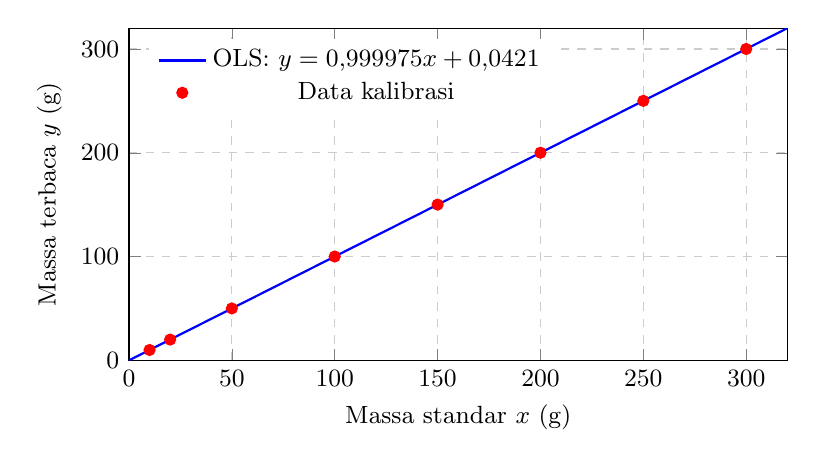
\begin{tikzpicture}
\begin{axis}[
  width=0.82\textwidth,height=5.8cm,
  xlabel={Massa standar $x$ (g)},ylabel={Massa terbaca $y$ (g)},
  xmin=0,xmax=320,ymin=0,ymax=320,
  grid=both,grid style={dashed,gray!40},
  legend pos=north west,legend style={font=\small,draw=none},
  tick label style={font=\small},label style={font=\small}]
\addplot[domain=0:320,samples=2,thick,blue]{0.999975*x+0.0421};
\addlegendentry{OLS: $y=0{,}999975x+0{,}0421$}
\addplot[only marks,mark=*,mark size=2pt,red]
  coordinates{(10,10.02)(20,20.03)(50,50.04)(100,100.06)(150,150.07)(200,200.05)(250,250.03)(300,300.01)};
\addlegendentry{Data kalibrasi}
\end{axis}
\end{tikzpicture}
\caption{Kurva kalibrasi neraca digital terhadap massa standar. Pada skala ini data dan garis OLS tampak berimpit, sehingga penyimpangan tidak terlihat; karena itu analisis residual diperlukan.}
\label{fig:cal}
\end{figure}

\begin{figure}[H]
\centering
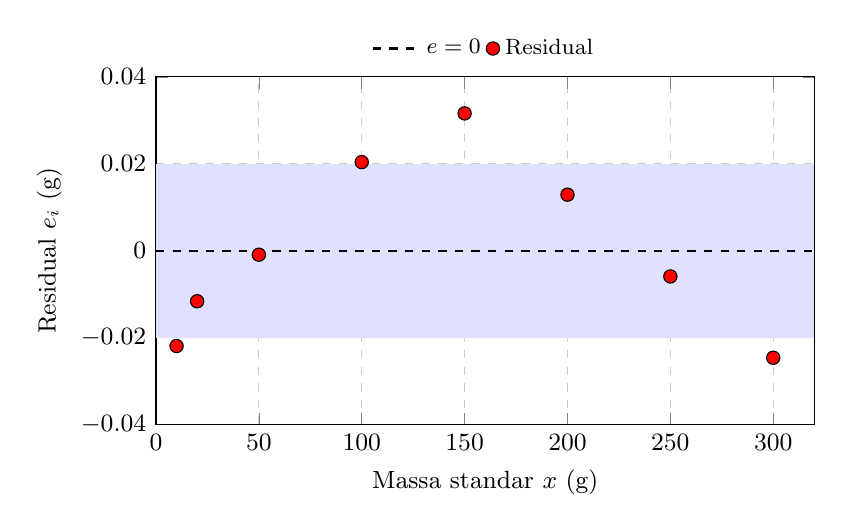
\begin{tikzpicture}
\begin{axis}[
  width=0.82\textwidth,height=6.0cm,
  xlabel={Massa standar $x$ (g)},ylabel={Residual $e_i$ (g)},
  xmin=0,xmax=320,ymin=-0.04,ymax=0.04,
  grid=both,grid style={dashed,gray!40},
  legend style={font=\footnotesize,draw=none,at={(0.5,1.02)},anchor=south,legend columns=-1},
  tick label style={font=\small},label style={font=\small},
  scaled y ticks=false,yticklabel style={/pgf/number format/fixed,/pgf/number format/precision=2}]
\fill[blue!12] (axis cs:0,-0.02) rectangle (axis cs:320,0.02);
\addplot[black,dashed,thick,domain=0:320,samples=2]{0};
\addplot[only marks,mark=*,mark size=2.4pt,red,draw=black]
  coordinates{(10,-0.0219)(20,-0.0116)(50,-0.0009)(100,0.0204)(150,0.0316)(200,0.0129)(250,-0.0059)(300,-0.0246)};
\legend{$e=0$,Residual}
\end{axis}
\end{tikzpicture}
\caption{Sebaran residual terhadap garis OLS. Pita biru menunjukkan batas $\pm\SI{0,02}{g}$ ($\approx 2\times$ resolusi). Empat dari delapan titik berada di luar pita, dan tandanya berpola $(-,-,-,+,+,+,-,-)$, yaitu bentuk busur terbalik.}
\label{fig:res}
\end{figure}

\begin{multicols}{2}
    \raggedcolumns
        \subsection{Lima Uji Validasi}
        Ringkasan lima uji validasi performa instrumen disajikan pada Tabel~\ref{tab:valid}.

        \subsection{Koreksi Hasil Pengukuran}
        Jika neraca dipakai tanpa koreksi, massa sejati dapat diperkirakan dari $x=(y-b)/a$. Untuk rentang \SIrange{10}{300}{g} koreksi ini berkisar \SI{0,01}{g} sampai \SI{0,07}{g}, atau lebih besar dari resolusi sehingga layak diterapkan pada pengukuran presisi.
\end{multicols}

%=== Tabel Lima Uji Validasi (Full Width) ===
\begin{table}[H]
\centering
\singlespacing
\caption{Ringkasan lima uji validasi performa instrumen.}
\label{tab:valid}
\small
\begin{tabularx}{\textwidth}{@{}l X X@{}}
\toprule
\textbf{Uji} & \textbf{Hasil} & \textbf{Penilaian}\\
\midrule
1. \textit{Accuracy} & Bias massa P1 $\SI{0,020}{g}$ ($0{,}030\%$); galat kalibrasi maksimum $+\SI{0,07}{g}$ pada \SI{150}{g} ($0{,}047\%$) & Dapat diterima untuk praktikum; bias $>U_m$ sehingga perlu koreksi\\
2. \textit{Repeatability} & $n=8$ (Group I): $s_r=\SI{0,0131}{g}$, $r=\SI{0,037}{g}$ & Baik, sekitar $1$ digit\\
3. \textit{Linearity} & Simpangan maks. $\SI{0,032}{g}$ ($0{,}011\%$ FS); residual berpola lengkung & Linier \textit{secara praktis} tetapi tidak acak murni\\
4. \textit{Functional} & Fungsi nol: pembacaan tanpa beban bergeser dari \SI{0,00}{g} menjadi \SI{0,03}{g} dalam $30$ menit sehingga \textit{zeroing} perlu diulang. Penguat: kemiringan $a=0{,}999975$ (selisih dari ideal $2{,}5\times10^{-5}$). \textit{Display}: pembacaan stabil pada dua desimal (\SI{0,01}{g}) dan fluktuasi antar-ulangan $\le\SI{0,04}{g}$ (rentang data massa P1 $67{,}20$--\SI{67,24}{g}) & Berfungsi baik; \textit{zeroing} perlu diulang berkala (simpulan dari data \textit{zero drift}, kalibrasi, dan \textit{repeatability})\\
5. \textit{Response/stability} & \textit{Zero drift} $+\SI{0,03}{g}/30$ menit; tunda gerbang cahaya $\approx\SI{0,8}{ms}$ (asumsi) & Perlu \textit{tare} berkala; tunda perlu dikoreksi\\
\bottomrule
\end{tabularx}
\end{table}

\begin{multicols}{2}
    \raggedcolumns
    \section{DISKUSI REFLEKTIF DAN INTEGRASI}
        \subsection{Analisis ``So What?'' Eksperimen P1}
        Hasil $\rho=(8{,}493\pm0{,}035)\ \si{g/cm^3}$ konsisten dengan kuningan, dan ketidakpastian relatifnya $0{,}41\%$. Implikasinya, pengukuran ini layak untuk mengidentifikasi bahan sebagai kuningan (bukan tembaga murni atau aluminium), tetapi tidak cukup untuk menentukan rasio Cu--Zn. Karena $85\%$ varians berasal dari diameter, mengganti jangka sorong (\SI{0,05}{mm}) dengan mikrometer sekrup (\SI{0,01}{mm}) menurunkan $U(\rho)$ dari $\SI{0,035}{g/cm^3}$ menjadi sekitar $\SI{0,026}{g/cm^3}$ (perkiraan dengan hanya $d$ diganti). Perbaikan sebanding pada $h$ membawanya ke sekitar $\SI{0,024}{g/cm^3}$. Perbaikan ini jauh lebih efektif daripada menambah jumlah pengulangan massa.

        \subsection{Analisis ``So What?'' Eksperimen M3: Kekekalan Energi}
        Hasil utama M3 adalah $\Delta E=(-2{,}79\pm0{,}61)\times10^{-3}\ \si{J}$. Nilai ini jauh dari nol, yaitu sekitar $4{,}6\,U$. Namun, tandanya negatif, artinya $E_2>E_1$: \textit{glider} seolah-olah memperoleh energi. Pada sistem dengan gesekan dan hambatan udara hal ini tidak mungkin secara fisis. Tafsir yang tepat bukan ``hukum kekekalan energi dilanggar'' dan bukan pula ``disipasi nyata terbukti'', melainkan bahwa \textbf{terdapat galat sistematis yang belum dikoreksi dan lebih besar daripada $U(\Delta E)$}.

        Beberapa kandidat penyebab dan uji kecukupannya:
        \begin{enumerate}
            \item \textbf{Response time delay.} Karena tunda $\tau$ membuat $v_2$ terlalu besar lebih jauh daripada $v_1$ (Tabel~\ref{tab:delay}), $E_2$ ter-\textit{overestimate} lebih banyak daripada $E_1$. Dengan $\tau=\SI{0,8}{ms}$ didapat $\Delta E=+\SI{0,97e-3}{J}$, atau berbalik menjadi disipasi positif yang masuk akal. Tanda $\Delta E$ menjadi nol tepat pada $\tau\approx\SI{0,59}{ms}$. Ini menunjukkan bahwa kecocokan sangat sensitif terhadap $\tau$ sehingga $\tau$ harus diukur dan bukan diasumsikan.
            \item \textbf{Ketidakakuratan $\Delta h$.} Agar $\Delta E=0$ tanpa koreksi $\tau$ diperlukan $\Delta h\approx\SI{29,4}{mm}$, atau lebih besar $\SI{1,4}{mm}$ dari yang tercatat. Selisih ini sekitar $18$ kali $U(\Delta h)$, sehingga kecil kemungkinan sebagai satu-satunya penyebab, tetapi kemiringan rel yang tidak seragam dapat berkontribusi.
            \item \textbf{Lebar \textit{flag} dan kecepatan sesaat.} $v=w/\Delta t$ adalah kecepatan rata-rata selama interupsi, bukan kecepatan di titik gerbang. Karena \textit{glider} dipercepat, kecepatan rata-rata berbeda sedikit dari kecepatan di titik tengah \textit{flag}, dengan pengaruh relatif lebih besar pada gerbang yang percepatannya mengubah $\Delta t$ lebih banyak.
        \end{enumerate}
        Disipasi nyata (gesekan lapisan batas udara dan pengereman arus pusar) pasti ada, tetapi dengan $\Delta E_{\text{terkoreksi}}\approx\SI{1e-3}{J}$ pada $\Delta s=\SI{0,80}{m}$ gaya disipatif rata-rata hanya sekitar $\SI{1e-3}{N}$, jauh di bawah yang dapat diselesaikan oleh $U(\Delta E)$ saat ini.

        \textbf{Implikasi:} pada eksperimen ini ketidakpastian acak ($U\approx\SI{6e-4}{J}$) sudah cukup kecil, tetapi galat sistematis dari instrumen (dinamis) mendominasi. Memperbanyak pengulangan tidak akan memperbaiki hasil; yang diperlukan adalah kalibrasi tunda sensor.

        \subsection{Komparasi Statis dan Dinamis}
        \begin{itemize}
            \item \textbf{Statis (P1):} galat didominasi galat acak dan resolusi ($\uA$ dan $\uB$ sebanding), sehingga dapat dikurangi dengan alat beresolusi lebih tinggi. Non-linieritas neraca bersifat kecil ($0{,}011\%$ FS) dan relevan terhadap bias, bukan terhadap $U(\rho)$.
            \item \textbf{Dinamis (M3):} galat didominasi galat sistematis ($\tau$) yang bergantung pada \textit{besaran waktu itu sendiri} sehingga makin besar pengaruhnya pada kecepatan tinggi. Galat ini lolos dari statistik $3\sigma$ dan tidak terlihat dari simpangan baku.
        \end{itemize}

    \section{KESIMPULAN DAN SARAN}
        \subsection{Kesimpulan}
        \begin{enumerate}
            \item Massa jenis silinder kuningan adalah $\rho=(8{,}493\pm0{,}035)\ \si{g/cm^3}$ ($k=2$). Diameter mendominasi ketidakpastian ($85\%$).
            \item Kalibrasi neraca menghasilkan $y=0{,}999975\,x+0{,}0421$ dengan $R^2\approx 1$, tetapi residual berpola lengkung (maksimum $\SI{0,032}{g}$), sehingga $R^2$ tidak boleh dipakai sendirian sebagai bukti linearitas.
            \item Pada M3, $\Delta E=(-2{,}79\pm0{,}61)\times10^{-3}\ \si{J}$ menunjukkan galat sistematis (terutama \textit{response time delay} gerbang cahaya), bukan pelanggaran kekekalan energi. Koreksi dengan $\tau=\SI{0,8}{ms}$ menghasilkan $\Delta E\approx+\SI{1,0e-3}{J}$ yang konsisten dengan disipasi kecil, tetapi nilai $\tau$ masih perlu diverifikasi.
            \item Galat dinamis sistematis lebih sulit dideteksi daripada galat statis acak, dan hanya dapat diatasi dengan kalibrasi dan koreksi, bukan dengan menambah pengulangan.
        \end{enumerate}

        \subsection{Rekomendasi Teknis}
        \begin{enumerate}
            \item \textbf{Ukur $\tau$ gerbang cahaya} dengan osiloskop dan sumber pulsa optik berpresisi mikrodetik, lalu terapkan koreksi $\Delta t_{\mathrm{sejati}}=\Delta t_{\mathrm{ukur}}+\tau$ di perangkat lunak pengolah data.
            \item \textbf{Gunakan mikrometer sekrup} untuk $d$ dan $h$ pada P1 guna menurunkan kontribusi dominan ketidakpastian $\rho$.
            \item \textbf{Perbaiki dan verifikasi kemiringan rel} (\textit{precision spirit level}, mis. $\SI{0,02}{mm/m}$) dan ukur $\Delta h$ dengan resolusi lebih halus dari \SI{0,1}{mm}.
            \item \textbf{Lakukan \textit{tare} berkala} dan koreksi kalibrasi neraca: ulangi kalibrasi dengan lebih dari $8$ titik (terutama di antara \SIrange{50}{200}{g}) untuk memodelkan kelengkungan, atau terapkan koreksi kuadratik.
            \item \textbf{Pasang \textit{draft shield}} (penutup akrilik) di lintasan rel dan hindari embusan AC langsung untuk mengurangi \textit{modifying inputs}.
            \item \textbf{Kalibrasi ulang berkala} dan catat suhu ruang, serta laporkan hasil selalu dalam bentuk $(\text{nilai}\pm U)$ dengan $k=2$.
        \end{enumerate}

    \section{DAFTAR PUSTAKA}
    \printbibliography[heading=none]

\end{multicols}

%======= Bagian Lampiran ===============
\onecolumn
    \newpage
    \begin{center}
        \section{LAMPIRAN}
    \end{center}

    \appendix

    \subsection*{Lampiran A: Rumus Excel yang Digunakan (Tanpa \textit{Hardcoding})}
    \noindent Sel yang dipakai pada sheet \texttt{Tab 2} (statistik P1 berada di kolom C--E, baris 6--13):

\begin{lstlisting}
n          : =COUNT('Tab 1 - Data Mentah'!B6:B13)
mean       : =AVERAGE('Tab 1 - Data Mentah'!B6:B13)
s          : =STDEV.S('Tab 1 - Data Mentah'!B6:B13)
uA         : =C8/SQRT(C6)
uB         : =C10/(2*SQRT(3))
uc         : =SQRT(C9^2+C11^2)
U (k=2)    : =2*C12
Volume V   : =(PI()/4)*D7^2*E7
rho        : =C7/C18
uc(rho)    : =C19*SQRT(C20^2+4*C21^2+C22^2)
U(rho)     : =2*C23
OLS slope  : =SLOPE(C5:C12,B5:B12)
OLS interc.: =INTERCEPT(C5:C12,B5:B12)
R^2        : =RSQ(C5:C12,B5:B12)
y_hat      : =$B$16*B5+$B$17        (sheet Tab 3)
residual   : =C5-D5
\end{lstlisting}

    \subsection*{Lampiran B: Anggaran Ketidakpastian $\Delta E$}
    \begin{table}[H]
    \centering
    \singlespacing
    \caption{Kontribusi tiap besaran terhadap $\uc(\Delta E)$ (pendekatan berkorelasi).}
    \label{tab:budgetE}
    \small
    \begin{tabular}{l S[table-format=1.2e-1] S[table-format=3.1]}
    \toprule
    \textbf{Sumber} & {Kontribusi$^2$ (J$^2$)} & {Porsi varians (\%)}\\
    \midrule
    $\Delta t_2$ & 7.32e-8 & 79.6\\
    $w$ & 8.25e-9 & 9.0\\
    $\Delta h$ & 5.96e-9 & 6.5\\
    $\Delta t_1$ & 4.56e-9 & 5.0\\
    $M$ & 1.13e-14 & 0.0\\
    \midrule
    \textbf{Total} & 9.20e-8 & 100.0\\
    \bottomrule
    \end{tabular}
    \end{table}

    \subsection*{Lampiran C: Ringkasan Skrip Python}
    \noindent Perhitungan dilakukan dengan \texttt{numpy}, \texttt{pandas}, \texttt{scipy}, dan \texttt{sympy} (turunan parsial simbolik untuk Persamaan~\eqref{eq:prop}), lalu diekspor ke Excel tiga tab dengan \texttt{openpyxl}. Berkas lengkap tersedia pada:
    \begin{itemize}
        \item Notebook: \texttt{Instrumentation\_Calibration\_Analysis.ipynb}
        \item Workbook: \texttt{Instrumentation\_Calibration\_Data.xlsx}
    \end{itemize}

    \subsection*{Lampiran D: Ringkasan Hasil Akhir Evaluasi}
    \begin{table}[H]
    \centering
    \singlespacing
    \caption{Ringkasan hasil akhir Group I ($k=2$).}
    \label{tab:ringkas}
    \small
    \begin{tabularx}{\textwidth}{@{}l X@{}}
    \toprule
    \textbf{Besaran} & \textbf{Hasil}\\
    \midrule
    Massa silinder $m$ & $(67{,}220\pm0{,}011)\ \si{g}$\\
    Diameter $d$ & $(2{,}0038\pm0{,}0038)\ \si{cm}$\\
    Tinggi $h$ & $(2{,}5100\pm0{,}0039)\ \si{cm}$\\
    Massa jenis $\rho$ & $(8{,}493\pm0{,}035)\ \si{g/cm^3}$\\
    Kecepatan $v_1$, $v_2$ & $(0{,}4798\pm0{,}0016)$ dan $(0{,}8985\pm0{,}0033)\ \si{m/s}$\\
    Energi $E_1$, $E_2$ & $(0{,}07798\pm0{,}00022)$ dan $(0{,}08077\pm0{,}00060)\ \si{J}$\\
    $\Delta E=E_1-E_2$ & $(-2{,}79\pm0{,}61)\times10^{-3}\ \si{J}$\\
    Regresi kalibrasi & $y=0{,}999975\,x+0{,}0421$; $R^2=0{,}99999997$; $s_{y/x}=\SI{0,0217}{g}$\\
    Residual maksimum & $\SI{0,032}{g}$ (berpola lengkung, tidak acak)\\
    \textit{Zero drift} & $+\SI{0,03}{g}$ per $30$ menit\\
    \bottomrule
    \end{tabularx}
    \end{table}

\end{document}
